\chapter{Conclusion}
\label{chapter:conclusion}

\section{Main conclusions}
In summary, the results obtained in the previous subchapters indicate that it is possible to perform semantically guided volumetric object manipulations using the chosen methodologies.

The experiments with the synthetic renderers (both 2D and 3D) demonstrate successes and failures when optimizing a differentiable renderer with respect to CLIP loss. If the optimization is only for a single parameter, there are viable alternatives to gradient descent. However, the benefit of using gradient descent becomes more pronounced when optimizing for multiple parameters - especially since the alternatives begin to perform progressively much worse as the parameter count increases. Many attempts were made to improve the stability of gradient descent, e.g. by augmenting the text prompts and rendered images. This had a measurable, but not entirely significant impact, and as such, the most deciding factor for the success of gradient descent remains to be the learning rate and starting point.

The NeRF manipulations appear to work to a certain degree, although the extent of how freely the object can be manipulated is limited by the bounds of the NeRF. As such, the manipulations will likely work better for NeRFs of a more unbounded nature. Also, there seems to be a few issues with the implementation - e.g. the "translucent" re-inserted flowers and the skewed z-rotation. However, these issues seem to be mostly code-related, since the re-insertion technique has been proven to work in \cite{benaim2022}.

\section{Future work}
\subsection{Text prompt augmentation}
A lot of work is currently being made in order to "unlock" the full potential of CLIP. In that regard, many are exploring the idea of \textit{prompt engineering}, which essentially revolves around rephrasing the text prompt to elicit different results from the model. Prompt engineering was explored a bit in \ref{sec:2d-semantic}, but it probably makes sense to perform these experiments in a more structured manner. 

On CLIP's official repository\footnote{\url{https://github.com/openai/CLIP}}, there is a notebook demonstrating how using various formulations involving the class name can improve the zero-shot classification capabilities of CLIP on ImageNet. For example, the formulations could be: "a bad photo of a {}.", "a cartoon {}.", "a jpeg corrupted photo of the {}.". These various formulations try to actuate some of the context regarding the text captions for the images in the dataset. A lot of these images are scraped from the internet, which is why they experiment with many prompts related to this origin (e.g. "a low resolution photo of {}.", "itap of {}." (itap is a subreddit), etc.). After compiling 80 of such templates, they proceeded to perform a sequential forward selection to determine which prompts performed the best on ImageNet. The search terminated after ensembling 7 templates. These templates are tried out for the 3D cow rendering example, producing the results seen in figure \ref{fig:4_cow-text-prompt-engineering}.
\begin{figure}[H]
    \centering
    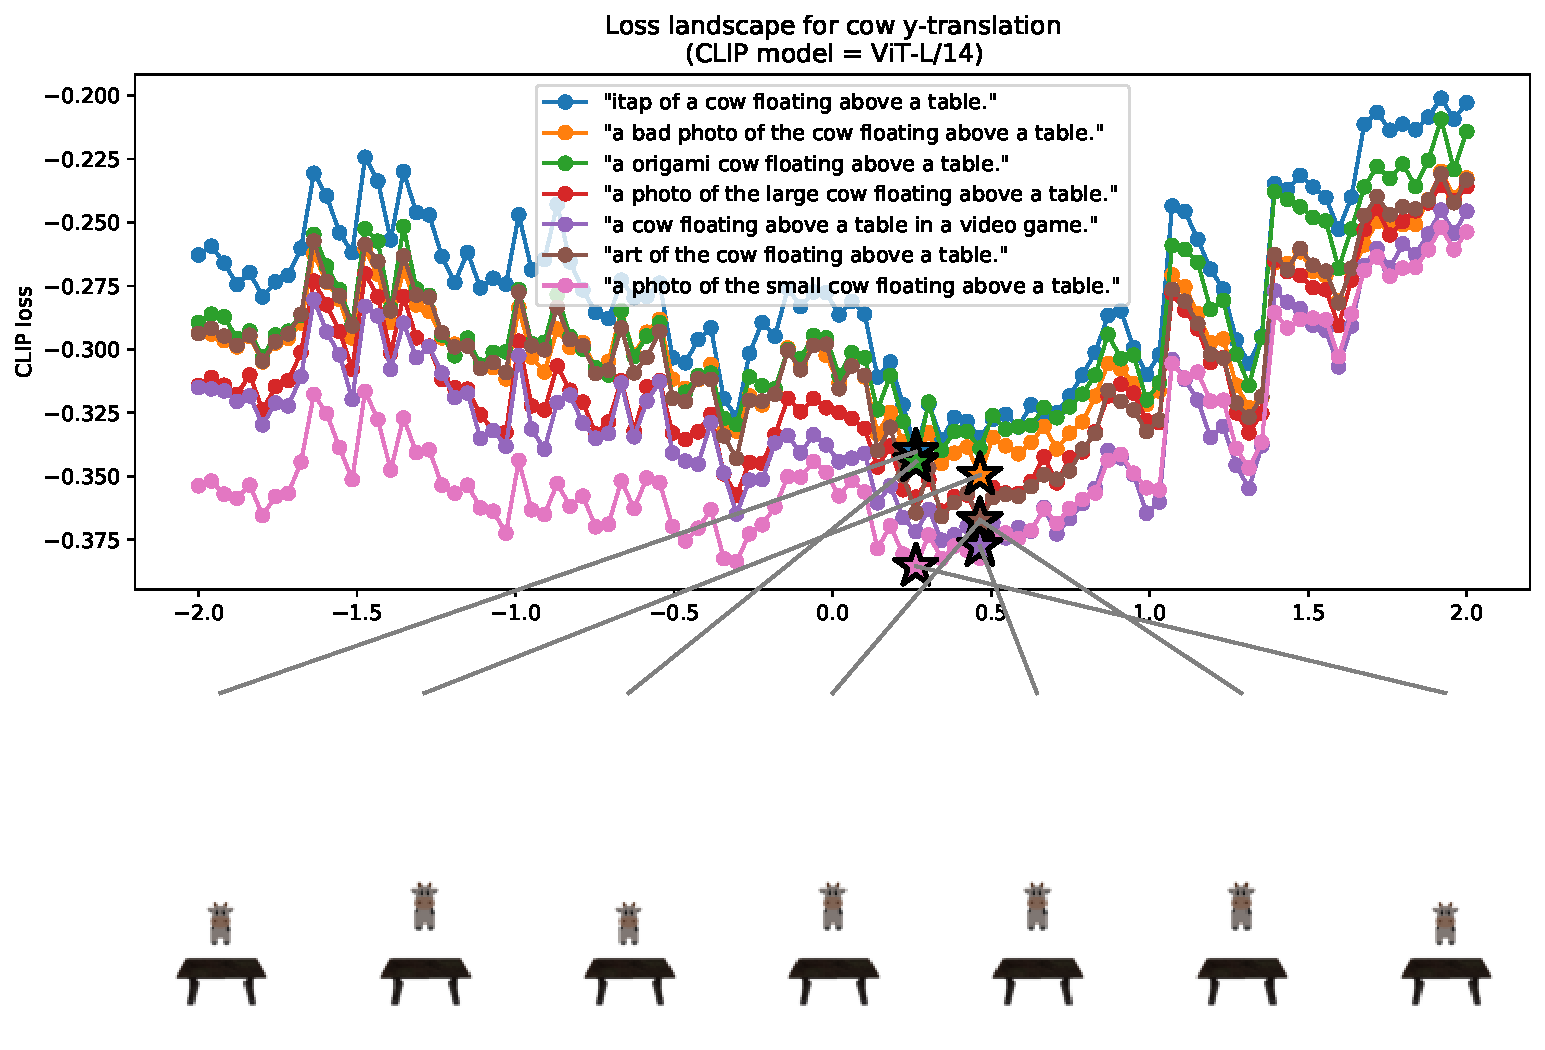
\includegraphics[width=1.0\textwidth]{figures/4_cow-text-prompt-engineering.pdf}
    \caption{Text prompt experiment for the 3D cow y-translation renderer. It seems like the shape of the landscape doesn't change much, but is instead uniformly shifted up/down.}
    \label{fig:4_cow-text-prompt-engineering}
\end{figure}

As mentioned in \ref{sec:2d-semantic}, it might also be worthwhile to try using an ensemble of CLIP models at once rather than using only a single version.

\subsection{Image augmentation} 
While many different variations of 2D image augmentation were experimented with in section \ref{sec:2d-semantic}, there was a method in particular which seemed promising (which wasn't mentioned in the section). It can be described as a sort of "Gaussian sampling" technique for obtaining augmented images. Given the transformation parameter(s) $\textbf{s}$, a fixed amount of perturbations $\textbf{N}$ are made in accordance to I.I.D samples from $\mathcal{N}(0,\sigma)$ (the reparameterization trick is applied here). The loss is then calculated as the mean of the losses for all the images. The mechanism is illustrated in figure \ref{fig:4_gaussian-sampling}, and the results from running gradient descent using the augmentation can be seen in figure \ref{fig:4_gaussian-sampling-gd}.
\begin{figure}[H]
    \centering
    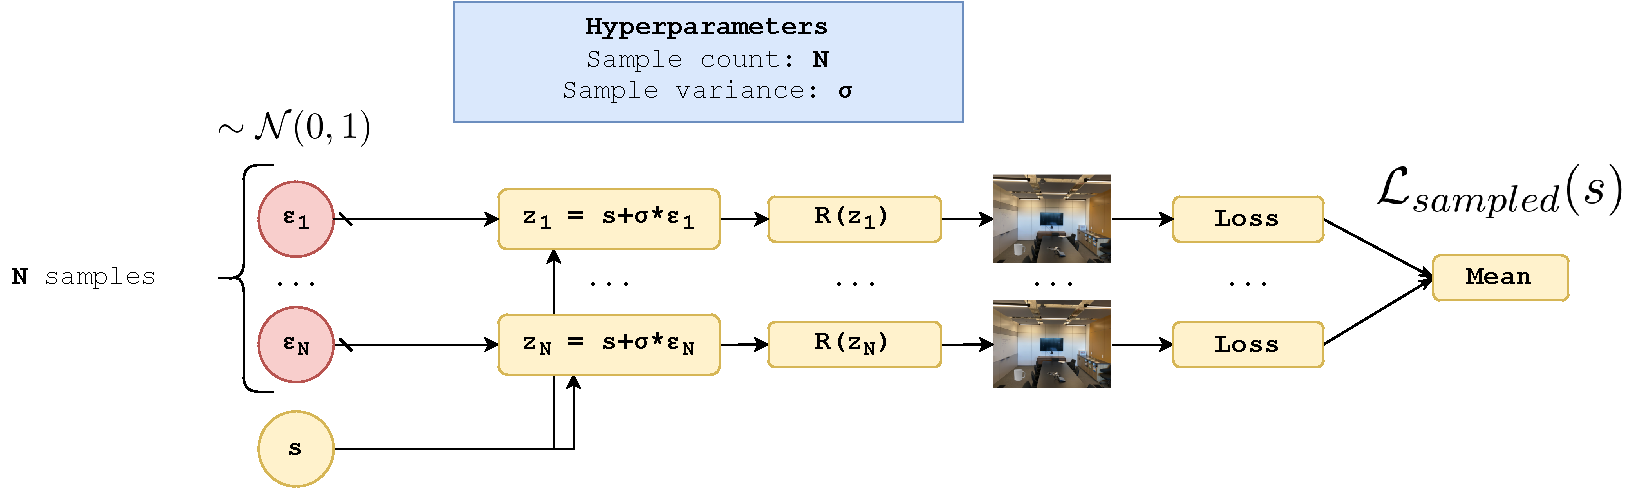
\includegraphics[width=1.0\textwidth]{figures/4_gaussian-sampling.pdf}
    \caption{"Gaussian sampling" method for image augmentation. Red nodes are stochastic (i.e. non-differentiable).}
    \label{fig:4_gaussian-sampling}
\end{figure}

\begin{figure}[H]
    \centering
    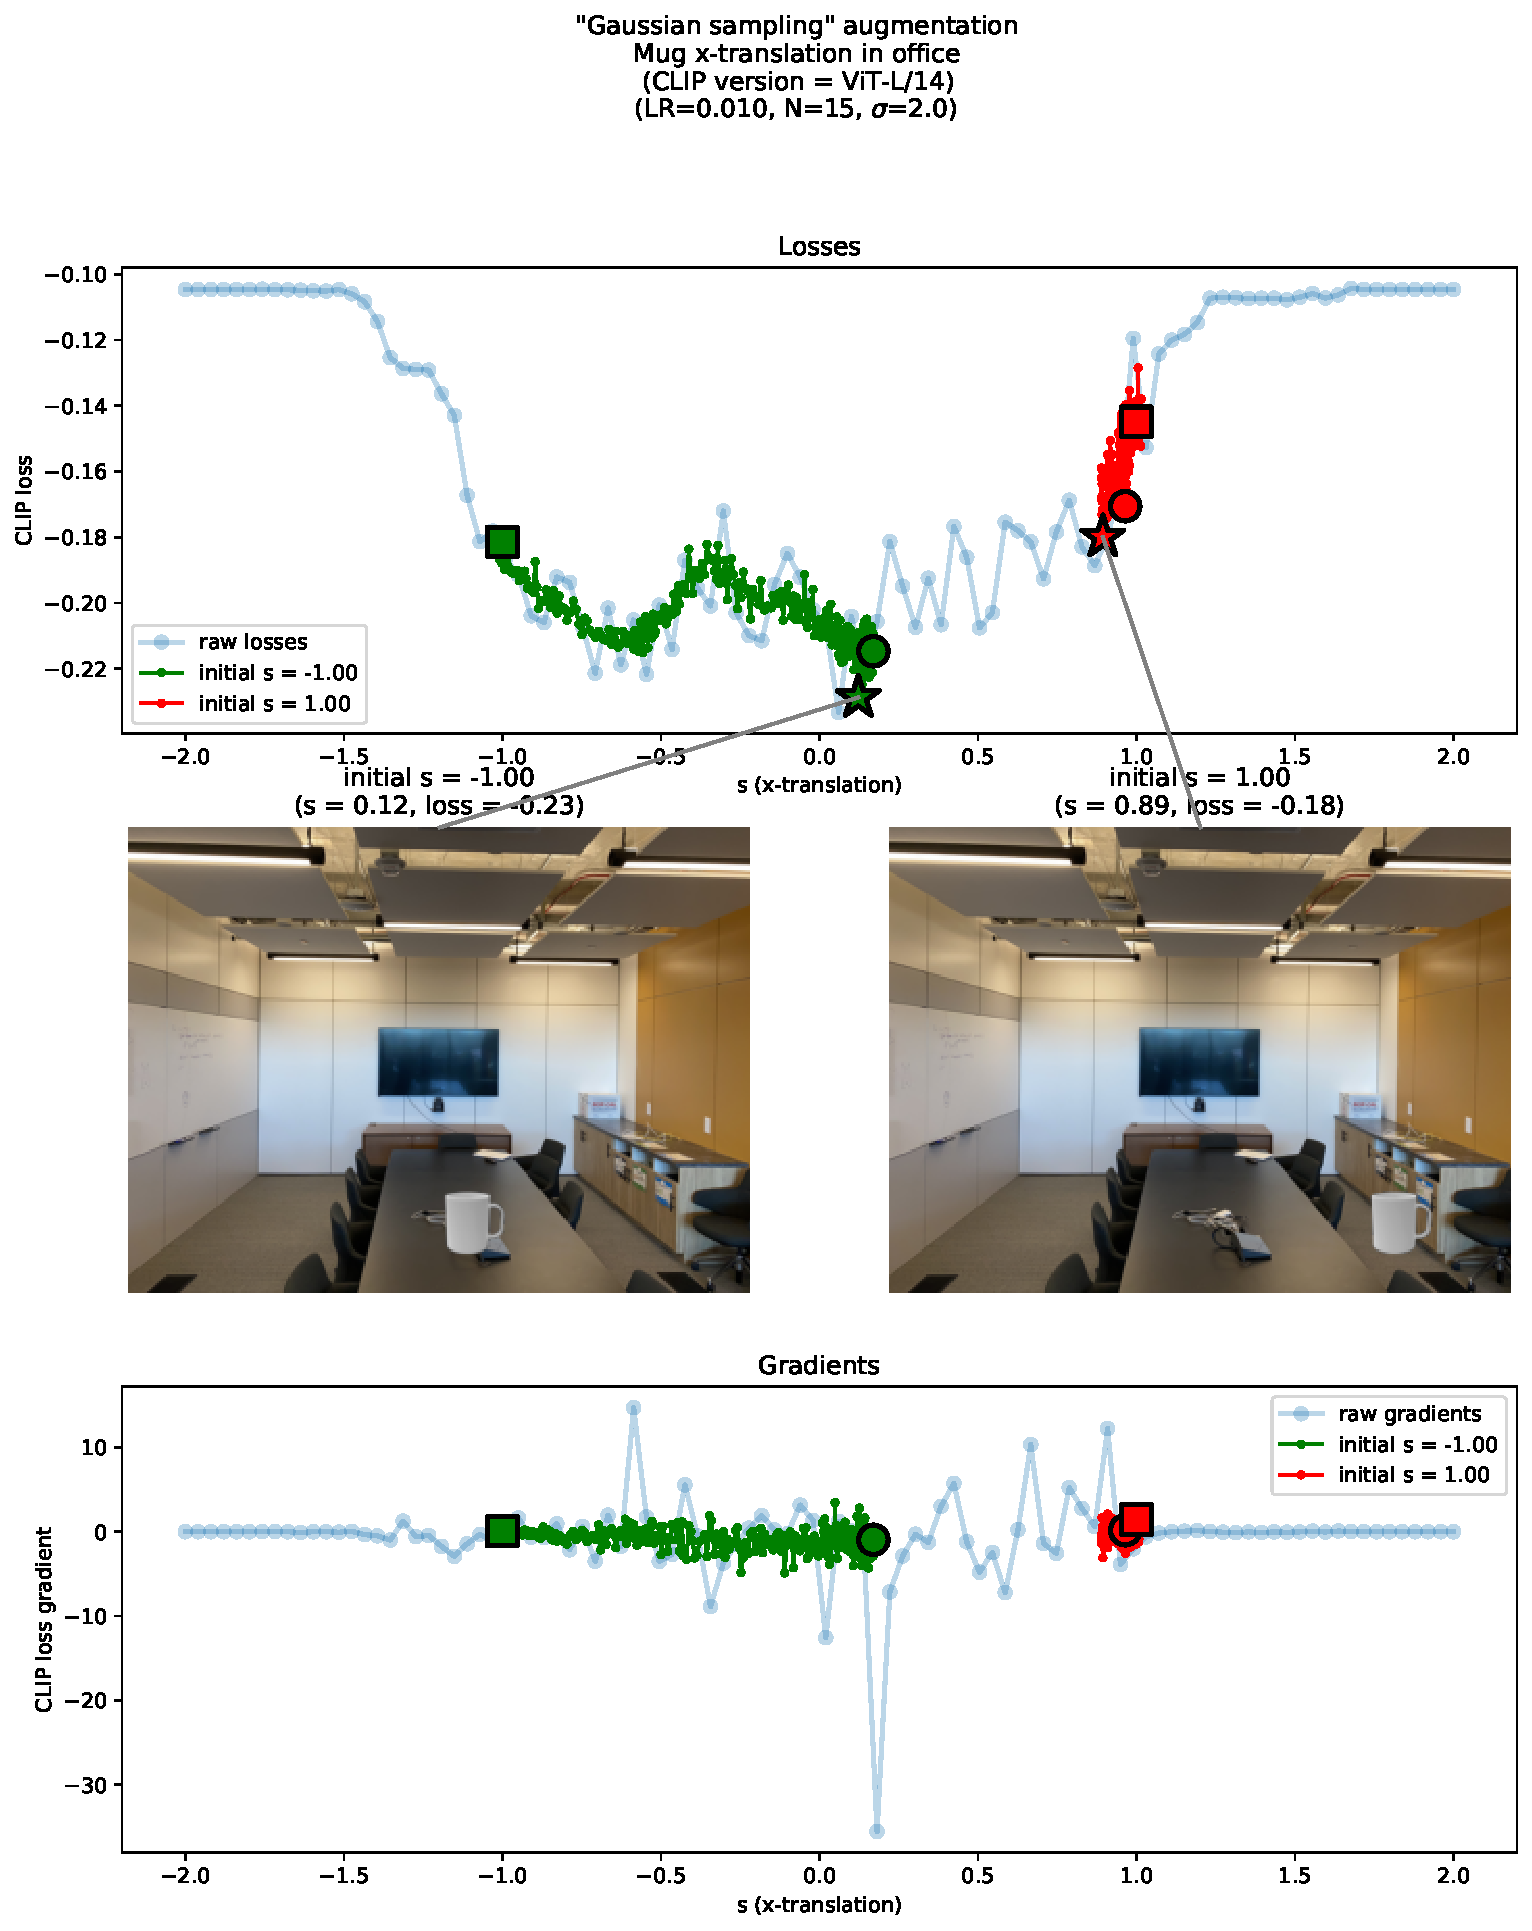
\includegraphics[width=1.0\textwidth]{figures/4_gaussian-sampling-gd.pdf}
    \caption{Gradient descent using the "Gaussian sampling" augmentation method. The top row shows the CLIP loss landscape overlaid with the gradient descent paths (the square is the starting point, the circle is the final point, the star is the minimum value encountered during training). The middle row shows the image corresponding to the minimum found during gradient descent. The bottom row shows the gradient values for the sample $s$-values.}
    \label{fig:4_gaussian-sampling-gd}
\end{figure}

In short, the results in figure \ref{fig:4_gaussian-sampling-gd} seem rather promising (it successfully descends into a good minimum for one of the starting points, and the gradient look much more smooth). Thus, for future work, it might be fruitful to perform further experiments with this particular type of augmentation.

\subsection{Hybrid optimization}
Even after many tricks, gradient descent is still rather imperfect, and the quality of the obtained solutions still depends a lot on the configuration (e.g. learning rate, schedule for learning rate, starting points, augmentation hyperparameters, etc.). It might make sense to draw inspiration from some of the gradient-free global optimizers that were experimented with in section \ref{sec:2d-optimization}. Maybe trying an ensemble of configurations and performing gradient descent multiple times could lead to finding better solutions.


\subsection{NeRF improvements}
There is definitely some room for improvement in regard to the \textit{torch-ngp} NeRF results. It could be worthwhile to investigate why the disentanglement did not work as expected. It might be important to uncover if the issue is code-related, or if disentanglement is fundamentally incompatible with that type of NeRF.

As for the flower NeRF results, there seemed to be some visual artifacts upon re-inserting the disentangled foreground object into the scene - even without performing any transformations. It's quite likely that the issue is code-related, since the methodology has been proven to work in \cite{benaim2022}. In my opinion, it definitely makes a lot of sense to figure out the reason behind this issue.

Also, given more time, it would have been very insightful to apply the disentanglement and manipulation to several other NeRF datasets. Currently, it cannot be entirely ruled out that the types of observed visual artifacts (e.g. the mosaic artifact) are specific to just the flower scene. Finding a dataset which is less bounded allow for greater manipulations in 3D space (e.g. rotate more freely, etc.).

\subsection{Object-centric transformations}
% object-centric intro
The NeRF transformations (specifically rotations) experimented with were all centered about the origin (i.e. [0,0,0]). If the goal is to rotate the object around itself, it requires that the 3D position of the foreground object be known (or at least estimated).
% propose solution
The idea was to research how a "centre-of-mass" method (such as the one proposed in the end of section \ref{sec:nerf-manipulation}) could be implemented. However, this was deemed out-of-scope since there were  issues with the regular NeRF transformations (i.e. visual artifacts appearing). In the future, this could be an interesting direction to take, since it allows for more granular manipulation of the object in the scene.

\subsection{Complete entire pipeline}
The main idea of this project was to combine CLIP-guided optimization and NeRF manipulations into a single pipeline. In practice, combining it all requires introduces a wide range of technical challenges in regard to code and hardware (specifically VRAM), which are beyond the scope of the project. Also, there are still existing issues which need to be resolved first (e.g. visual artifacts from transformations).


